\section{Introduction}

XML~\cite{XML} (eXtensible Markup Language) is a standard language for organizing
and representing semi-structured (tree-structured) data, and it has been
widely used for decades.
The success of XML has led to a great many applications that have been
specially developed for XML. Among them, XPath~\cite{XPath} is a query expression language for XML,
and it uses a path expression to specify a set of XML elements.
XPath is also the basis of other query languages such as XQuery.

In the last decade, the rapid growth of the amount of information has led to
an urgent demand for high-performance data processing technologies for
business and scientific research.  
When the size of XML data exceeds the size we can deal with 
by conventional DOM-based tools, we need more involved techniques
such as parallelization in distributed-memory environments or stream processing.

When we compute in parallel in distributed-memory environments, we first
need to divide the input into smaller parts and allocate them to the
computers.  One possible approach is to adopt a tree-dividing technique
for the tree that an XML document represents.  A naive way is to divide
a tree at the root or at a fixed depth, but this does not guarantee the
size of subtrees.  A more involved way is to apply the $m$-bridge
technique~\cite{mbridges}~\cite{mbridges1} with which we can divide a tree into parts no
larger than the parameter $m$.  However, these tree-based divisions
require parsing the whole XML document in advance, and this may limit the applications.

In this paper, we propose another approach for input division in which
we divide the XML document (text).  Usually, XML data are stored in the serialized format,
and it is very easy to divide a text into smaller chunks.
It is, however, not trivial to apply queries for those chunks because
some necessary information to applying queries is missing in a chunk.

To clarify the problem, consider that the input is the following XML document
and a chunk is given from the underlined part.
\begin{quote}\small\tt
\smallskip
<A><B><C>c1</C><C>c\underline{2</C><C>c3</C><A><C>c4</C><B>}\\
</B></A></B><A><B></B></A><B></B></A>
\smallskip
\end{quote}
Fig.~\ref{fig:example} shows the tree structure that the XML document represents.
Here comes a fundamental question.  \emph{What structure does
the chunk represent\/}? The chunk includes tags (beginning
and/or end tags), which are gray in Fig.~\ref{fig:example}. Note
that some tags, such as the first \verb|</C>| or the last \verb|<B>|,
miss their matching tags. It seems that we cannot obtain the structure and that it is impossible 
to apply the query to a randomly split chunk.

To solve this problem, we add some nodes from the root of the tree and
formalize the idea as a \emph{partial tree} as shown in
Fig.~\ref{fig:partialtree} (the figure has four different types of
nodes, which will be discussed in detail in
Section~\ref{sec:partialtree}).  
By adding the nodes on the path from the root, we are now able to apply
the queries based on the parent-child relationships.  

\begin{figure}[t]
\centering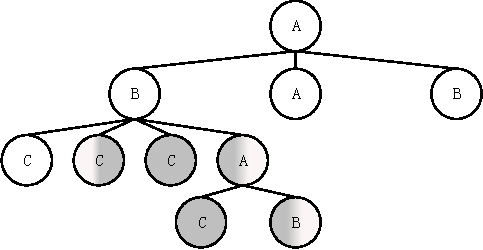
\includegraphics{partialtree/figures/fromWord-1.pdf}
\caption{An example XML tree}
\label{fig:example}
\end{figure}

\begin{figure}[t]
\centering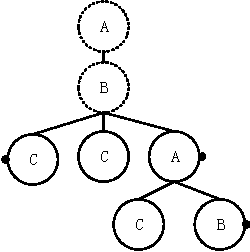
\includegraphics{partialtree/figures/fromWord-3.pdf}
\caption{Partial tree for the example.}
\label{fig:partialtree}
\end{figure}

In this paper, we deal with an important subset of XPath queries called
\emph{navigational XPath queries}~\cite{xpathcategory} in which we specify the nodes with not only
the parent-child relationships but also the inter-sibling relationships
and additional conditions called predicates.  Although a partial tree has
the parent-child relationships from the root, it lacks the information
required to process navigational XPath queries, a node may have only some
of its children, and some siblings may be on another partial tree.
Therefore, we develop a new algorithm for processing navigational XPath
queries over a set of partial trees with communication.
Our algorithm is easy to implement because it processes the steps in a query (including those in predicates) 
one by one and is efficient because we carefully analyzed the conditions to reduce the communication among partial trees.

The contributions of our study are summarized as follows.

\begin{itemize}
\item \textbf{Formalizing the structure for XML chunks}:
We first formalize the structure and properties of partial trees that are given from chunks of an XML document (Section~\ref{sec:partialtree}). We also show an algorithm to parse the chunks and construct the partial trees (Section~\ref{sec:construction}).

\item \textbf{Parallelizing XPath Queries}:
We then develop an algorithm for executing the navigational XPath queries in parallel (Section~5).
Basically, the algorithm runs independently on partial trees, but it also performs communication
to obtain the correct query results.

\item \textbf{Experiments on GB-level XML documents}:
We implemented the algorithm in Java and conducted experiments on a PC cluster with GB-level XML documents (Section~6).  Our implementation successfully processed an 8 GB XML document in parallel and obtained speedups of a factor of 6.0 over 16 PCs.
\end{itemize}


The remainder of the paper is organized as follows. In Section 2, we review the XPath query. In Section 3, we discuss the partial trees in detail. In Section 4, we discuss how to construct partial trees from chunks of an XML document. In Section 5, we discuss executing XPath query  algorithms in parallel. We 
report the experiment results in Section 6. Related work is shown in Section 7, and we conclude the paper in Section 8.


% LocalWords: kmatsu 
